\documentclass[11pt,a4paper]{report}

\usepackage[utf8]{inputenc}
\usepackage[T1]{fontenc}

\pagestyle{empty}

\usepackage{graphicx}% Include figure files
%\usepackage{epstopdf}
%\usepackage{pdfsync}
\usepackage{amstext,amsbsy}
\usepackage{times} 

%% Numbered problems
\newcounter{excount}[chapter]
\newenvironment{exercise}[1][]{\addtocounter{excount}{1} \noindent {\bf Problem
    \arabic{excount} \ \ #1}\hspace{2mm}}{\vspace{4mm}}


\title{FYS3120 Classical Mechanics and Electrodynamics\\ 
\vspace{15mm}Problem set 1}


%%%%%%%
\begin{document}
%%%%%%%
\maketitle

%%%%%%%%
\begin{exercise}
Figure~\ref{fig:gc} shows four different mechanical systems, in {\bf a)} a pendulum attached to a block which in turn is attached to a spring, {\bf b)} a pendulum which is attached to a vertical ring which rotates with a fixed frequency $\omega$, {\bf c)} a straight rod which can tilt without sliding on the top of cylinder, while the cylinder can roll on a horizontal plane (no slipping), and {\bf d)} a spinning top which moves on a horizontal floor.

\begin{figure}[h!]
\begin{center}
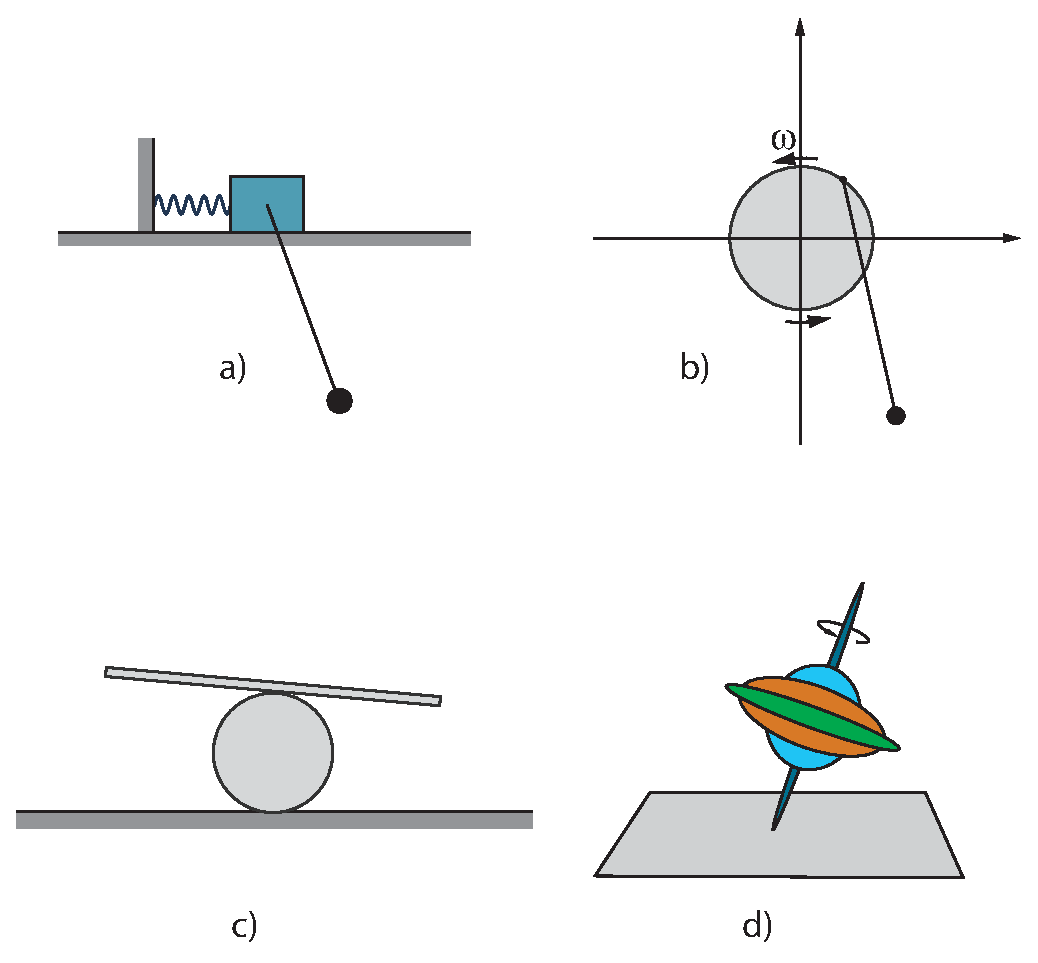
\includegraphics[width=0.9\textwidth]{Fig1-1.eps}
\end{center}
\caption{Four mechanical systems.}
\label{fig:gc}
\end{figure}

In all cases specify the number of degrees of freedom and choose an appropriate set of generalized coordinates.
\end{exercise}
%%%%%%%%


%%%%%%%%
\begin{exercise}
An Atwood machine consists of three parts, with masses $m_1=4m$, $m_2=2m$ and $m_3=m$, that move vertically, and two rotating pulleys, which we treat as massless.  The fixed lengths of the ropes, which we also consider as massless, are $l_1$ and $l_2$. We show the set-up in Fig.~\ref{fig:atwood}.

Explain why the number of degrees of freedom of the system is two and choose a corresponding set of generalized coordinates. Find the potential and kinetic energies of the system expressed as functions of the generalized coordinates and their time derivatives. Write down the Lagrangian of the system.

%%%%%%%%%%
\begin{figure}[h!]
\begin{center}
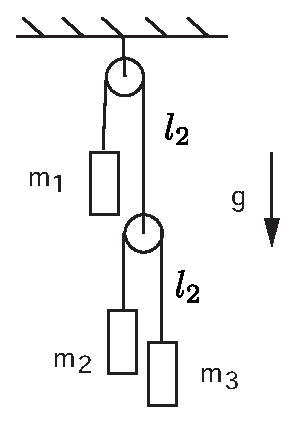
\includegraphics[height=5cm]{Atwood.eps}
\end{center}
\caption{An Atwood machine with three weights.}
\label{fig:atwood}
\end{figure}
%%%%%%%%%% 

\end{exercise}
%%%%%%%%


\newpage
%%%%%%%%
\begin{exercise}
Three identicals rods of mass $m$ and length $l$ are connected by frictionless joints and suspended,  with the distance between the points of suspension being equal to the length of the rods, as shown in Fig.~\ref{fig:rods}. The rods move in the plane. Explain why the system has only one degree of freedom, and choose the angle $\theta$ as generalized coordinate.

%%%%%%%%%% 
\begin{figure}[h!]
\begin{center}
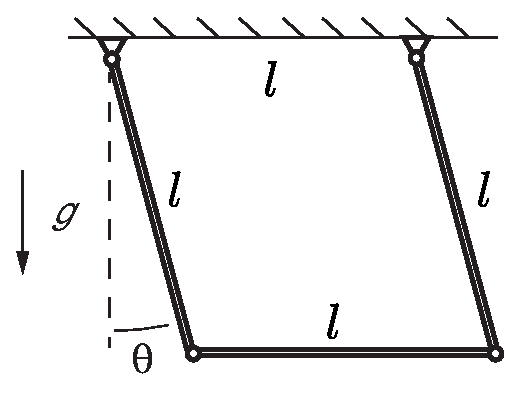
\includegraphics[width=5cm]{ThreeRods.eps}
\end{center}
\caption{System of moving suspended rods.}
\label{fig:rods}
\end{figure}
%%%%%%%%%% 

Show that the Lagrangian, defined as the difference between the kinetic and potential energy, $L=K-V$, gets the following form as a function of $\theta$ and $\dot\theta$,
\begin{equation}
L(\theta,\dot\theta)={5\over 6}m l^2\dot\theta^2+2mgl\cos\theta.
\end{equation}
We remind you that the expression for the moment of of inertia of a rod about its endpoint is $I={1\over 3}m l^2$.
\end{exercise}
%%%%%%%%


%%%%%%%%
\begin{exercise}
A particle with mass $m$ moves in three-dimensional space under the influence of a constraint. The constraint is expressed by the equation
\begin{equation}
e^{-(x^2+y^2)}+z=0,
\end{equation}
for the Cartesian coordinates $(x,y,z)$ of the particle.
\begin{itemize}
\item[\bf a)]Explain why the number of degrees of freedom of the particle is two. Use $x$ and $y$ as generalized coordinates and find the expression for the position vector $\vec r$ of the particle in terms of $x$ and $y$. 
\item[\bf b)]A virtual displacement is a change in the position of the particle $\vec r \to \vec r + \delta \vec r$ which is caused by an inifinitesimal change in the generalized coordinates, $x \to x + \delta x$ and $y\to y+\delta y$. Find $\delta \vec r$ expressed in terms of $\delta x$ and $\delta y$.
\item[\bf c)]The constraint can be interpreted as a restriction for the particle to move on a two-dimensional surface in three-dimensional space. Any virtual displacement $\delta \vec r$ is a tangent vector to the surface while the constraint force $\vec f$ which acts on the particle is perpendicular to the surface. Use this to determine $\vec f $ (up to a normalization factor) as a function of $x$ and $y$.
\item[\bf d)]Make a drawing of a section through the surface for $y=0$. Indicate in the drawing the direction of the two vectors $\vec f$ and $\delta \vec r$ for a chosen point on the surface.
\end{itemize}
\end{exercise}
%%%%%%%%

%%%%%%%%%
%\begin{exercise}
%A flexibel chain can move without friction on a smooth surface, as shown in Fig.~\ref{fig:chain}. It has constant mass density along the chain. The vertical heigths of the end points are $z_A$ and $z_B$. Use the principle of virtual work to find how $z_A$ and $z_B$ are related when the chain is in static equilibrium.
%
%\begin{figure}[h!]
%\begin{center}
%\includegraphics[width=7cm]{VirtualWork.eps}
%\end{center}
%\caption{Flexible chain.}
%\label{fig:chain}
%\end{figure}
%
%\end{exercise}
%%%%%%%%


%%%%%%
\end{document}
%%%%%%%%
